\documentclass[a4paper,11pt]{article}
\usepackage[utf8]{inputenc}
\usepackage[T1]{fontenc}
\usepackage[english]{babel}
\usepackage{graphicx}
\graphicspath{{./}}
\usepackage{booktabs}
\usepackage{amsmath}
\usepackage{siunitx}
\title{TP3: Modelling the Human Eye}
\author{Rong ZHOU}
\newcommand{\univaddress}{3 Rue Augustin Fresnel, 57070 Metz}
\date{\today}
\newcommand{\contact}{ron@ronzz.org}

\begin{document}
\maketitle

\section{Introduction}

The human eye is probably one of the finest constructions of nature. Equipped with a lens capable of changing focal distance from about 250~mm to infinity with the aid of the rectus muscles, our eye perceives things from far just like from close-up. In this experiment, we seek to reconstruct the human eye with an optical bench to better understand the function of the human eye from an optical physics perspective, notably how the eye is able to adjust itself to focus on objects close-up and far away.

\section{Experimental Setup}

For this experiment, we employ the following equipment:

\begin{itemize}
    \item an optical bench with graduations
    \item a point light source emitting diverging light rays
    \item a transparent gridded glass serving as object
    \item converging lenses with nominal focal distances at 10, 15 and 20~cm
    \item a blank screen
    \item various mounts to affix the optical equipment to the bench
\end{itemize}

\section{Experimental Procedure}

\subsection{Verification of actual focal distances of converging lenses by autocollimation}

First, we verify the focal distances of the converging lenses to be employed in our experiment with the following setup:

\begin{figure}[h]
\centering
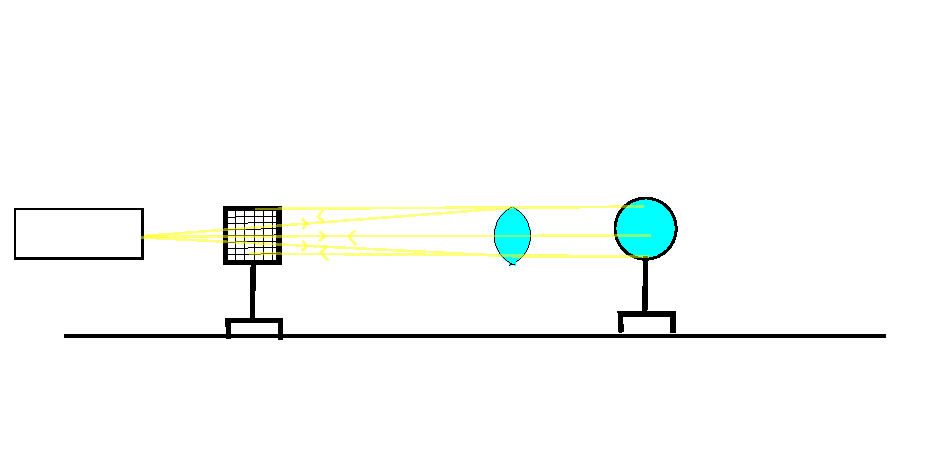
\includegraphics[width=0.9\linewidth]{autocollimation-refined.pdf}
\caption{Autocollimation setup for focal distance verification}
\label{fig:autocollimation}
\end{figure}

We obtained the following results:

\begin{table}[h]
\centering
\begin{tabular}{lrrr}
\toprule
 & \multicolumn{3}{c}{Lens} \\
\cmidrule{2-4}
 & 1 & 2 & 3 \\
\midrule
Nominal focal distance (mm) & 100 & 150 & 200 \\
Measured focal distance (mm) & 104 & 155 & 208 \\
\bottomrule
\end{tabular}
\caption{Nominal vs.\ measured focal distances}
\label{tab:focal-distances}
\end{table}

\subsection{Construction of a fictitious eye}

We construct a fictitious eye with a converging lens, which represents the lens in the eye, and a blank screen, which represents the retina:

\begin{figure}[h]
\centering
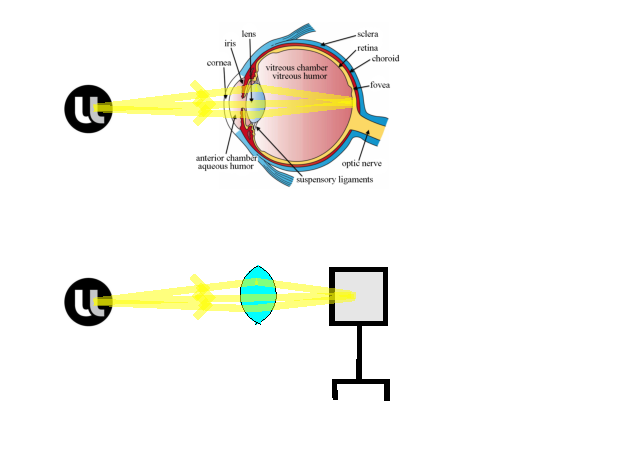
\includegraphics[width=0.9\linewidth]{eye-model.pdf}
\caption{Model of the fictitious eye}
\label{fig:eye-model}
\end{figure}

\subsubsection{Focus on an object at infinity}

We construct a scenario simulating the focus on an object considered infinitely far away (light rays arriving in parallel):

\begin{figure}[h]
\centering
\includegraphics[width=0.9\linewidth]{eye-vision-infinity.pdf}
\caption{Fictitious eye focused at infinity}
\label{fig:eye-infinite-focus}
\end{figure}

\subsubsection{Focus on a nearby object (200 mm)}

We construct a scenario simulating the focus on an object 200~mm away from the eye:

\begin{figure}[h]
\centering
\includegraphics[width=0.9\linewidth]{eye-vision-closeup.pdf}
\caption{Fictitious eye focused on an object 200~mm away}
\label{fig:eye-closeup-focus}
\end{figure}

With Descartes' law
($\frac{1}{\overrightarrow{AO}} + \frac{1}{\overrightarrow{OA'}} = \frac{1}{\overrightarrow{OF'}}$),
we calculated the new focal distance required to obtain a clear image on the ``retina'' to be 104~mm, which is experimentally verified as a clear image is obtained when we replaced the converging lens of a nominal focal distance of 200~mm (``eye lens'') with a converging lens of a nominal focal distance of 100~mm.

\subsection{Experimentation with magnifying glasses to understand the mechanism of optical magnification}

After having constructed the fictitious eye and understood its optical mechanisms, we now with the aid of converging lenses (which serve as magnifying glasses) attempt to understand the mechanisms of optical magnification.

The experimental setup is as follows:

\begin{figure}[h]
\centering
\includegraphics[width=0.9\linewidth]{magnifying-glass.pdf}
\caption{Experimental setup with magnifying glass}
\label{fig:magnifying-glass}
\end{figure}

Hence we have $O_{\text{eye}}A = 600~\text{mm}$ (arbitrary choice), eye focused on infinity (simulated with converging lens of $f_{\text{nominal}} = 200~\text{mm}$).

With the aid of a ruler, we have measured the size of 11 vertical grids of the gridded glass to be 24~mm, which translates into an average of 2.182~mm per grid.
For convenience, we isolate the four grids above the focal centre, which has a theoretical height of 8.727~mm as our object ($AB = 8.727~\text{mm}$):

\begin{figure}[h]
\centering
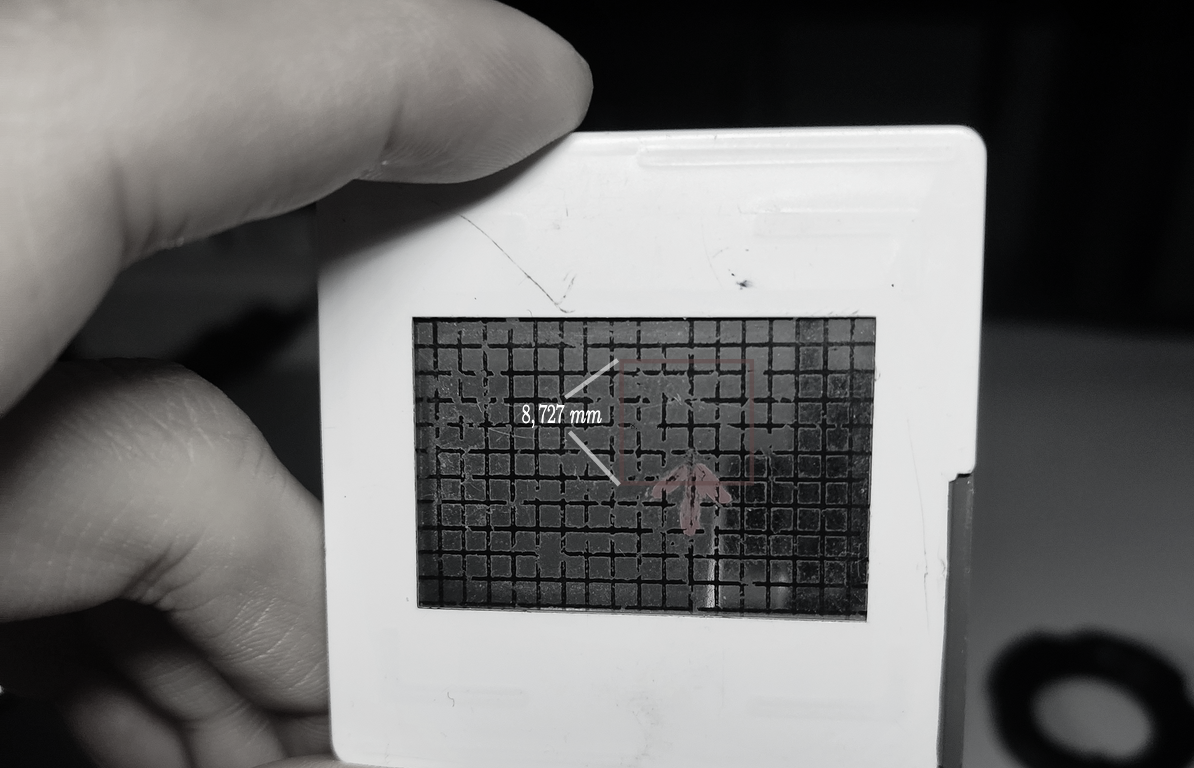
\includegraphics[width=0.9\linewidth]{grid-glass.png}
\caption{Gridded glass used as object, with four grids isolated above the focal centre}
\label{fig:grid-glass}
\end{figure}

This translates to an observation angle $\alpha$ of approximately 0.0145 radians:

\begin{figure}[h]
\centering
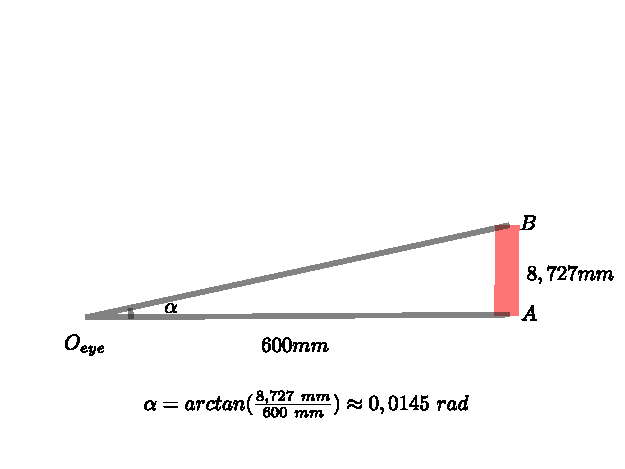
\includegraphics[width=0.9\linewidth]{observation-angle-object.pdf}
\caption{Observation angle $\alpha$ of the object}
\label{fig:observation-angle-object}
\end{figure}

To observe the magnification effect, we place converging lenses of various focal lengths between the ``eye lens'' and the object $AB$, moving them around until a clear image is obtained. We note this position as $O$. $AB$ designates the object (4 vertical grids), and $A'B'$ designates the image projected onto the ``retina''.

Since the eye is focused at infinity, the light rays arriving at the ``eye lens'' must be parallel to form a clear image on the ``retina''. Therefore, $\alpha' = \arctan\!\left(\frac{AB}{AO}\right)$. So the magnification magnitude $M = \frac{\alpha'}{\alpha} = \frac{\arctan\!\left(\frac{AB}{AO}\right)}{0.0145~\text{rad}}$:

\begin{figure}[h]
\centering
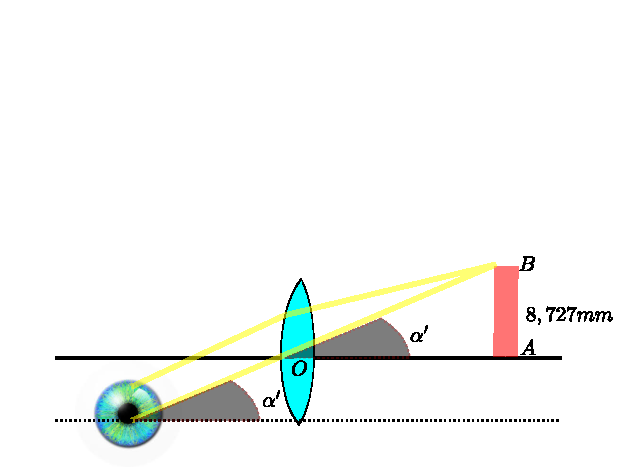
\includegraphics[width=0.9\linewidth]{magnification-magnitude.pdf}
\caption{Diagram of the magnification magnitude $M$}
\label{fig:magnification-magnitude}
\end{figure}

Experimentally we have obtained the following measurements:

\begin{table}[h]
\centering
\renewcommand{\arraystretch}{1.4}
\begin{tabular}{lrrrr}
\toprule
Measurement & \multicolumn{4}{c}{Magnifying glass} \\
\cmidrule{2-5}
 & 1 & 2 & 3 & 4 \\
\midrule
Nominal focal distance $f$ (mm) & 100 & 150 & 300 & 500 \\
$OA$ (mm) & 142 & 186 & 260 & 392 \\
$A'B'$ (mm) & 9.0 & 7.7 & 6.0 & 5.0 \\
$\frac{A'B'}{AB}$ (calculated) & 1.031 & 0.882 & 0.688 & 0.573 \\
$M$ (calculated) & 4.22 & 3.22 & 2.31 & 1.53 \\
$\frac{M}{\frac{A'B'}{AB}}$ & 4.092 & 3.654 & 3.356 & 2.671 \\
\bottomrule
\end{tabular}
\caption{Experimental magnification measurements}
\label{tab:magnification}
\end{table}

From which we can attest that the human eye lens ``shrinks'' images before passing them to the retina. As we noticed the field of vision (which is represented by the number of visible grids on the screen) is increasingly limited with higher magnification magnitudes, we infer that this is by design to preserve the field of vision while we look at objects way larger than our eye!

In addition, graphing $M$ against $\frac{1}{f}$:

\begin{figure}[h]
\centering
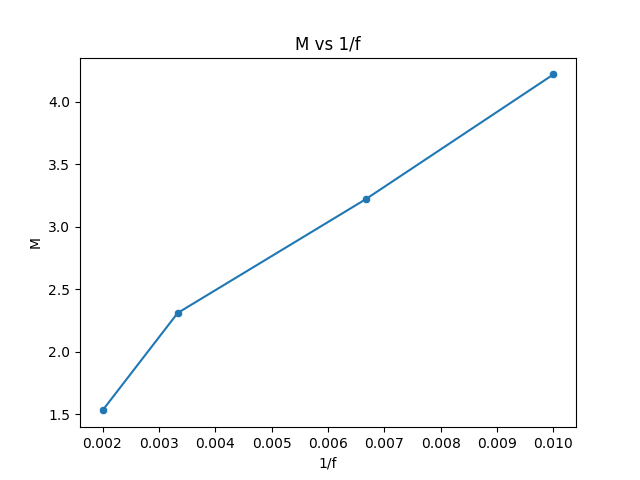
\includegraphics[width=0.9\linewidth]{M-f.png}
\caption{Graph of magnification $M$ vs.\ $\frac{1}{f}$}
\label{fig:M-f}
\end{figure}

We witness a near-linear relationship between the two, as expected.

\section{Conclusion}

In this experiment, we reconstructed a human eye with optical geometric analogs to understand how a human eye is able to focus on objects of different distances. We then placed converging lenses of various focal lengths in front of our physical analog eye to understand the functioning of magnifying glasses. Our experimental results concur with theoretical derivations.

\section{Bibliography}

\begin{thebibliography}{99}
\end{thebibliography}

\section{Appendix}

Python code used to graph $M$ against $\frac{1}{f}$:

\begin{verbatim}
import seaborn as sns
import matplotlib.pyplot as plt
import pandas as pd

# Your data (converted to proper floats)
data = pd.DataFrame({
    "inv_f": [0.01, 0.00666666666666667, 0.00333333333333333, 0.002],
    "M": [4.22, 3.22, 2.31, 1.53]
})

# Plot
sns.scatterplot(data=data, x="inv_f", y="M")

# Optional: add line
sns.lineplot(data=data, x="inv_f", y="M")

plt.xlabel("1/f")
plt.ylabel("M")
plt.title("M vs 1/f")
plt.show()
\end{verbatim}

\end{document}
